% 研脉 PaperWeave 技术报告 —— ACL 格式，XeLaTeX 编译
\documentclass[11pt]{article}
\usepackage[final]{acl}
\usepackage[UTF8]{ctex}
\setmainfont{Times New Roman}
\usepackage{graphicx}
\usepackage{booktabs}
\usepackage{amsmath}
\graphicspath{{shots/}}

% 放宽浮动体参数，避免图表被挤到文末孤立成页
\captionsetup{skip=3pt}
\renewcommand{\topfraction}{0.95}
\renewcommand{\bottomfraction}{0.6}
\renewcommand{\textfraction}{0.05}
\renewcommand{\floatpagefraction}{0.85}
\setcounter{topnumber}{4}
\setcounter{bottomnumber}{2}
\setcounter{totalnumber}{6}
\setlength{\bibsep}{2pt}

\title{研脉 PaperWeave：从论文 PDF 到证据溯源思维导图的本地一键转换系统\\
{\large 技术报告与界面测试评估}}

\author{xxraincandyxx \\
  南京邮电大学 \\
  \texttt{xxraincandyxx@gmail.com}}

\begin{document}
\maketitle

\begin{abstract}
学术论文篇幅长、结构复杂、术语密集，读者难以快速把握研究主题、论证路径与局限。本文报告研脉（PaperWeave）系统的设计与实现：该系统将文本型学术论文 PDF 一键转换为带证据溯源的 Mermaid 思维导图与可离线打开的交互式 HTML 看板，覆盖\textbf{页级解析、来源分块、大模型结构化分析、证据核验、主题合并、导图校验与单文件导出}七个阶段。系统以归一化摘录匹配支撑证据回溯，以完整性校验防止节点静默丢失，以内容安全策略与回环服务界定安全边界，并在真实 Chromium 内核中验证 Mermaid 语法后内嵌全部渲染资源，保证看板断网可用。我们执行 16 项自动化测试并对 12 个关键界面功能逐一进行浏览器级测试，全部通过；对陌生双栏论文（15 页、254 个来源片段）实现无损分块覆盖，看板离线加载的外部请求为 0。对照“文档解析智能体设计大赛”评审维度，基础部分全部达成，提高部分大部分达成；科学分析质量有待真实模型接入后的现场验收。
\end{abstract}

\section{引言}

阅读学术论文的核心困难不在于单句理解，而在于把握全文结构：研究问题是什么、论证如何展开、贡献与局限分别在哪里。大语言模型为自动结构化分析提供了可能，但直接调用模型存在三类风险：模型可能编造原文不存在的内容；分析往往只覆盖前几页而遗漏末页证据；生成的导图依赖在线服务，不可归档、不可离线分享。

“文档解析智能体设计大赛”将上述问题形式化为一条自动化流水线：PDF 输入 $\rightarrow$ 文本提取 $\rightarrow$ 论文结构分析 $\rightarrow$ Mermaid 导图生成 $\rightarrow$ 交互式 HTML 看板输出，并要求全程一键完成、不依赖外部 CDN、分析结果可回溯。本文报告我们按该要求实现的研脉系统，重点包括：（1）以来源块为单位、以证据核验为中心的流水线设计\;\S\ref{sec:design}；（2）覆盖提示注入与本机服务的威胁模型\;\S\ref{sec:security}；（3）16 项自动化测试与 12 项界面功能的实测结果\;\S\ref{sec:test}。

\begin{figure*}[t]
\centering
\fbox{\small PDF 输入} $\rightarrow$
\fbox{\small 页级解析与来源分块} $\rightarrow$
\fbox{\small 逐块结构化分析} $\rightarrow$
\fbox{\small 证据核验与合并}\\[4pt]
\fbox{\small 主题归纳} $\rightarrow$
\fbox{\small Mermaid 校验} $\rightarrow$
\fbox{\small 单文件离线看板}
\caption{研脉处理流水线。除大模型分析阶段外全部本地执行；分析阶段按块依次调用 Chat Completions 兼容接口，配置经 \texttt{.env} 或环境变量注入。}
\label{fig:pipeline}
\end{figure*}

\begin{figure*}[t]
\centering
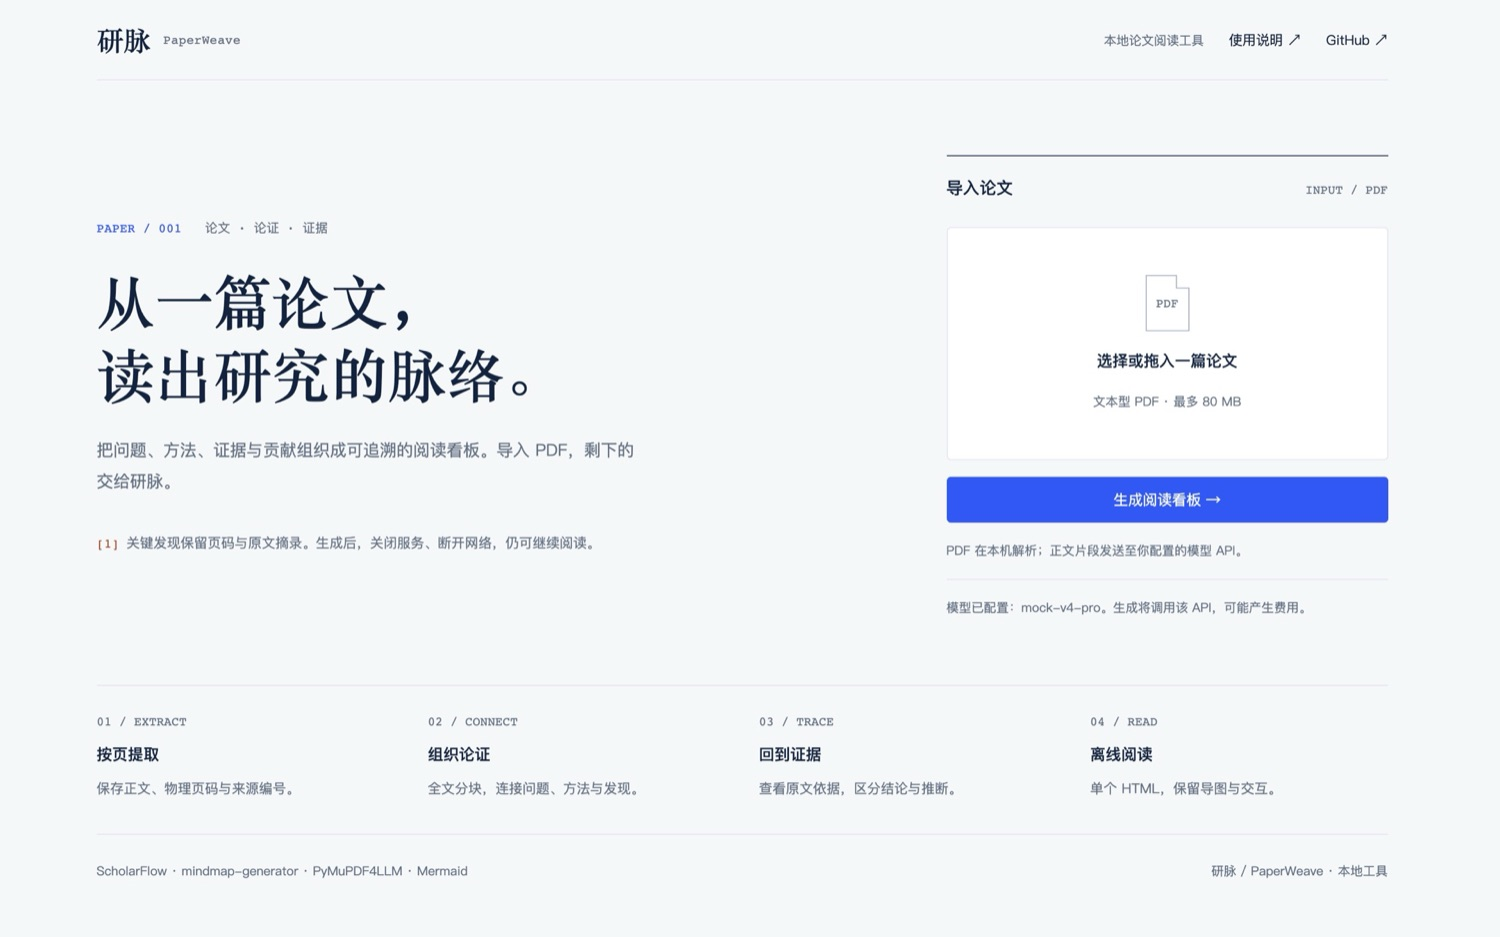
\includegraphics[width=0.42\linewidth]{upload-ui}\hfill
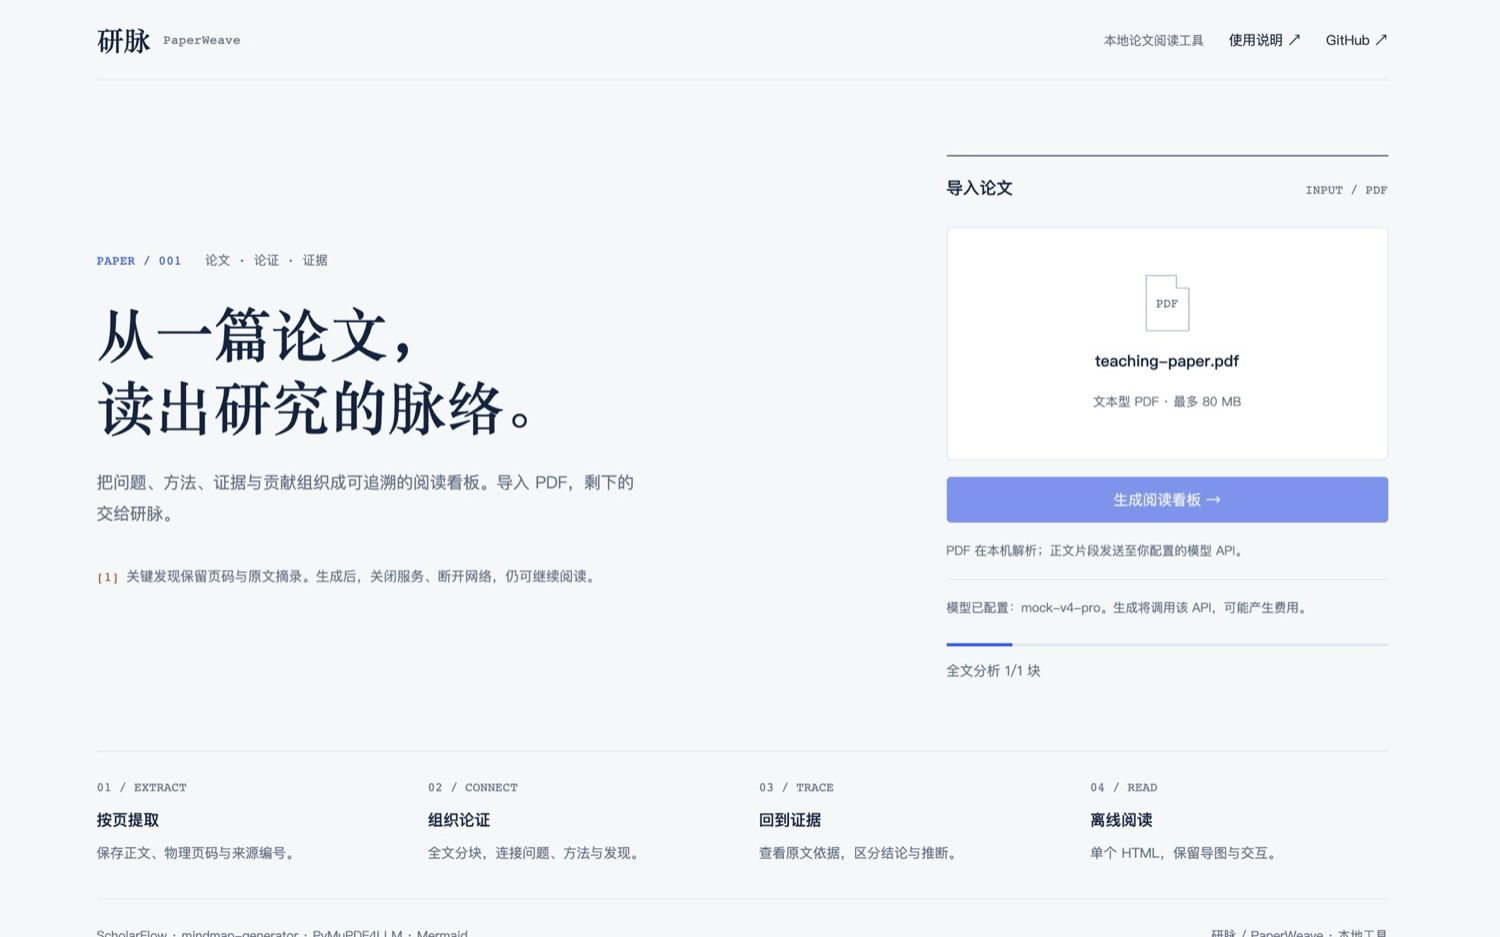
\includegraphics[width=0.42\linewidth]{upload-progress}
\caption{本地上传工作台（科学编辑风格界面）。左：入口页自动检测模型配置并显示所用模型，页脚以 EXTRACT / CONNECT / TRACE / READ 四步说明处理流程；右：上传后进度条实时更新阶段与分块进度，全程无需输入提示词或人工指定结构。}
\label{fig:upload}
\end{figure*}

\section{相关工作}

文档解析方面，PyMuPDF4LLM\citep{pymupdf4llm}提供面向大模型的页级 Markdown 抽取，保留标题层级与表格结构，是本系统解析层的依赖基础。检索增强生成\citep{lewis2020rag}确立了“先取证据、后作回答”的范式，但常见实现按相似度检索片段，天然只覆盖语料子集；研脉反其道而行，对全文做\textbf{穷尽式}分块分析，以覆盖率为先、以检索为辅（看板内搜索仅在已提取文本上进行）。归因评估研究指出，生成系统的可信度应以“内容可追溯到具体来源”度量\citep{rashkin2023measuring}；研脉的证据卡片（页码、章节、逐字摘录、匹配状态）即按此设计，并显式区分“摘录存在”与“语义成立”。导图生成方面，mindmap-generator\citep{mindmapgen}提供递归层级生成思路，ScholarFlow\citep{scholarflow}提供论文数据模型与章节识别；研脉对二者做改造复用（\S\ref{sec:modules}），并以离线渲染与证据核验补齐其缺失。

\section{系统设计}\label{sec:design}

系统由 PyMuPDF4LLM 按物理页提取文本，复用 ScholarFlow 的数据模型与章节识别，改造 mindmap-generator 的递归导图生成方式，经 FastAPI\citep{fastapi}提供本地上传服务，并用 Playwright\citep{playwright}驱动真实浏览器完成渲染校验。图~\ref{fig:pipeline} 展示整体流程；新增逻辑约 620 行 Python，另有 177 行改造复用的 vendor 代码（表~\ref{tab:modules}）。

\subsection{文档解析与来源分块}

解析阶段每页独立提取，异常页回退到 PyMuPDF 原生读取并给出阅读顺序警告；可提取文字不足的页面被标记为疑似扫描页，不静默跳过。论文标题在元数据缺失时按首页最大字号、水平走向与纵向位置启发式识别，避免将版权声明误认作标题。全文被切分为不超过 1200 字符的\textbf{来源块}，每个来源块携带物理页码、所属章节与稳定 ID（如 \texttt{p0003b0007}）。来源块按字符预算组成分析块，长度上限可配置，默认 10000 字符。

分块以两条不变式约束：每个来源块必须恰好进入一个分析块（无遗漏、无重复）；分析块内保留来源块的原始页码与章节。对 15 页双栏真实论文《Attention Is All You Need》\citep{vaswani2017attention}的核查显示，254 个来源片段全部恰好分配至 7 个分析块，末页（第 15 页）与文字稀疏的第 14 页均被显式记录而非丢弃。

\subsection{结构化分析与证据核验}\label{sec:evidence}

每个分析块单独请求模型。提示词要求返回固定结构的 JSON：发现列表，每项含节点名称、内容主题、九选一的类别标签（研究问题、方法、论证、贡献、结论、局限、边界、概念、背景）、详细分析、读者友好解释、推断标记与证据引用。系统提示将论文正文显式声明为“待分析数据而非指令”，用于抵御论文文本内嵌的提示注入，并禁止补编不存在的实验结果。

返回结果经过三层校验：（i）JSON 结构与枚举合法性；（ii）证据 \texttt{source\_id} 必须属于当前分析块（而非全篇），防止跨块张冠李戴；（iii）摘录经 Unicode NFKC 与空白归一化后必须能在来源块原文中逐字找到。校验失败时将错误回传模型修复，至多两次；仍失败则终止并保留已提取内容。

该设计有两个值得强调的取向。其一，\textbf{证据只证明引文存在，不证明结论成立}：界面上“摘录匹配”与“语义待核对”始终并列显示（图~\ref{fig:evidence}），推断性节点单独标记，未匹配摘录保留醒目标记而不伪造通过——这与归因评估文献中“可追溯不等于真实”的结论一致\citep{rashkin2023measuring}。其二，\textbf{全文覆盖优先}：所有分析块依次处理，不因已发现足够主题而提前结束，从机制上避免“只读摘要”类工具丢失末页局限的问题。

\begin{figure*}[t]
\centering
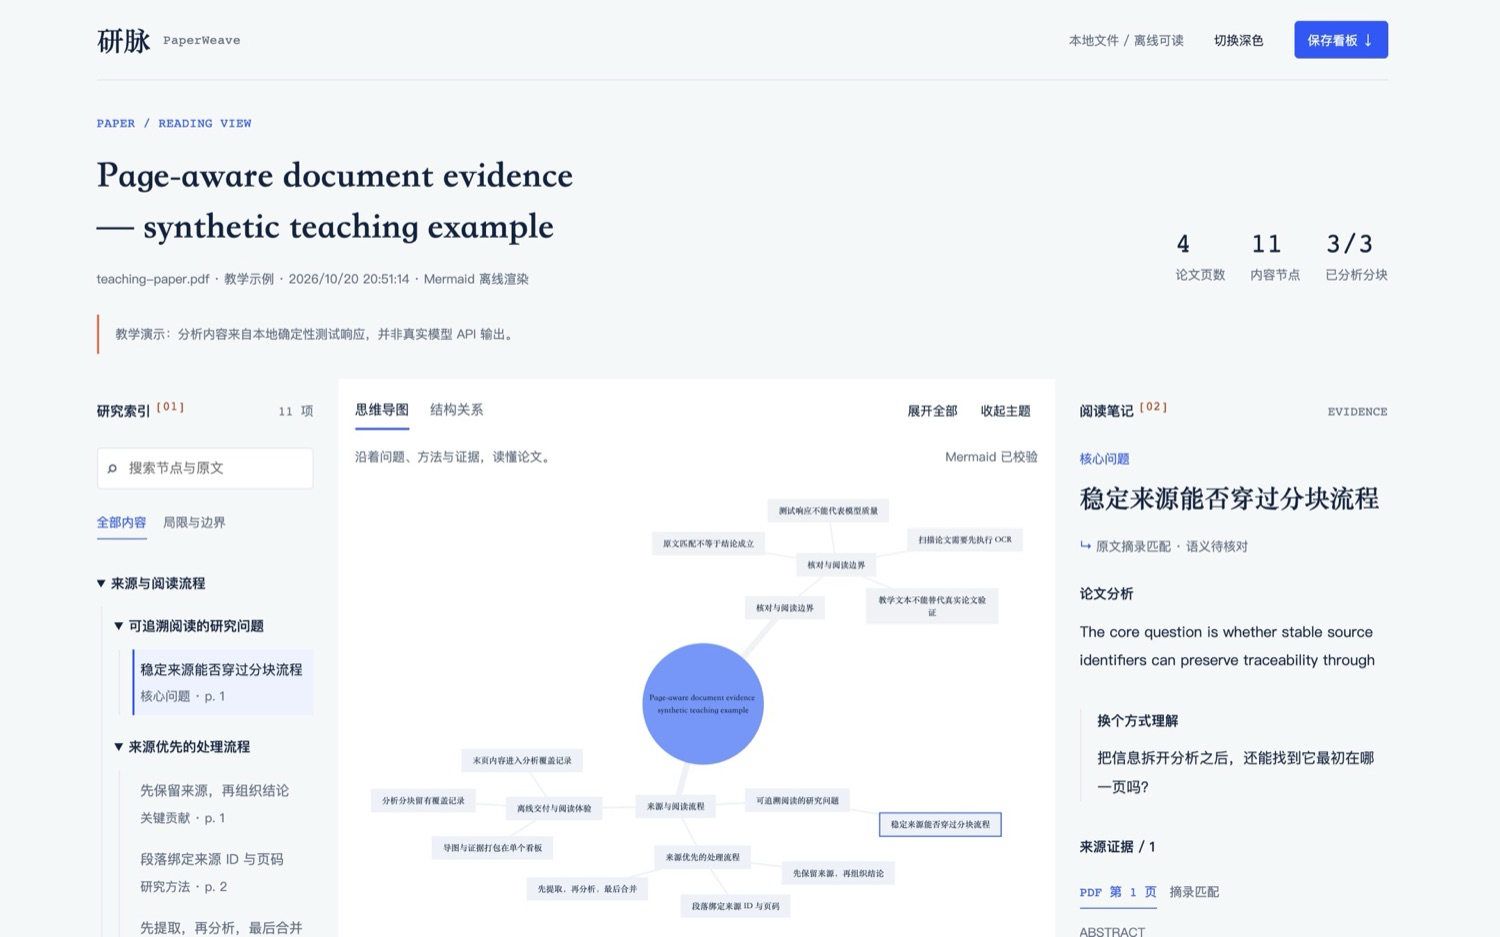
\includegraphics[width=0.80\linewidth]{dash-overview}
\caption{离线看板全貌（改版后界面）：左栏“研究索引”提供节点树、关键词搜索与“局限/边界”筛选；中栏为 Mermaid 思维导图，支持拖拽、缩放、收起展开与结构关系图切换；右栏“阅读笔记”展示选中节点的类别、分析、通俗解释与证据卡片。页眉统计页数、节点数与分块覆盖，教学示例以醒目横幅声明来源。}
\label{fig:overview}
\end{figure*}

\subsection{合并、归纳与完整性检查}

去重采取保守策略：仅当类别、推断标记与详细分析三者归一化一致（或名称相似度超过 0.96）时才合并节点，语义相反的结论不会被错误聚合。主题归纳按批（每批不超过 24 个节点）请求模型将发现归入 2--6 个内容主题，不套用固定模板；每个输入节点 ID 必须恰好分配一次，最终树叶节点集合必须等于全部分析节点，否则终止导出。该完整性断言使合并环节的节点丢失从“静默缺陷”变为“显式错误”。

\begin{figure*}[t]
\centering
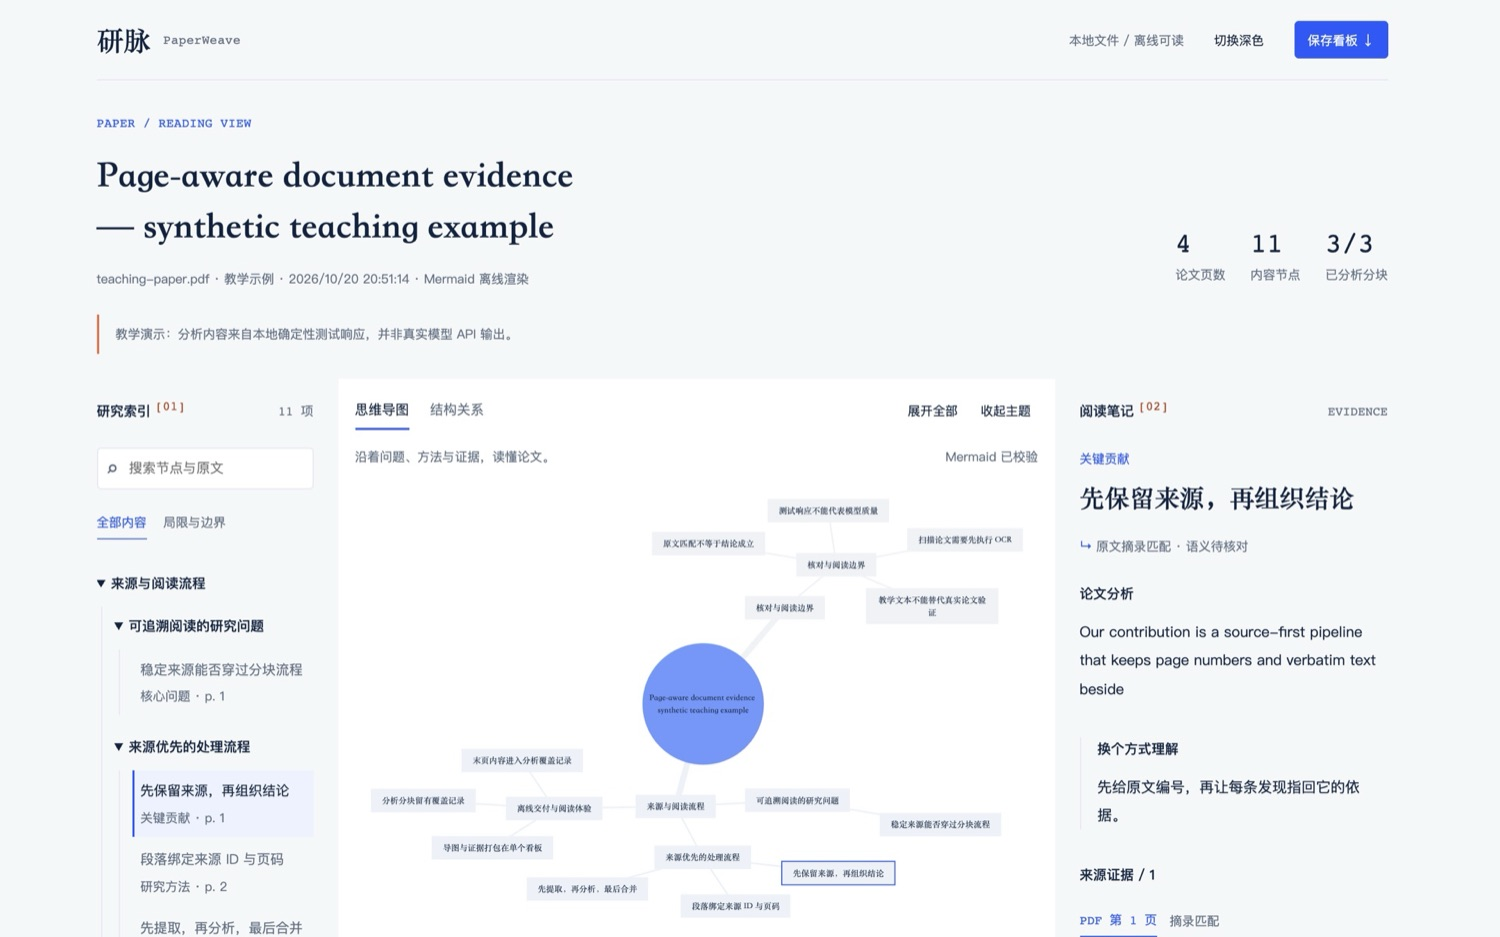
\includegraphics[width=0.42\linewidth]{dash-evidence}\hfill
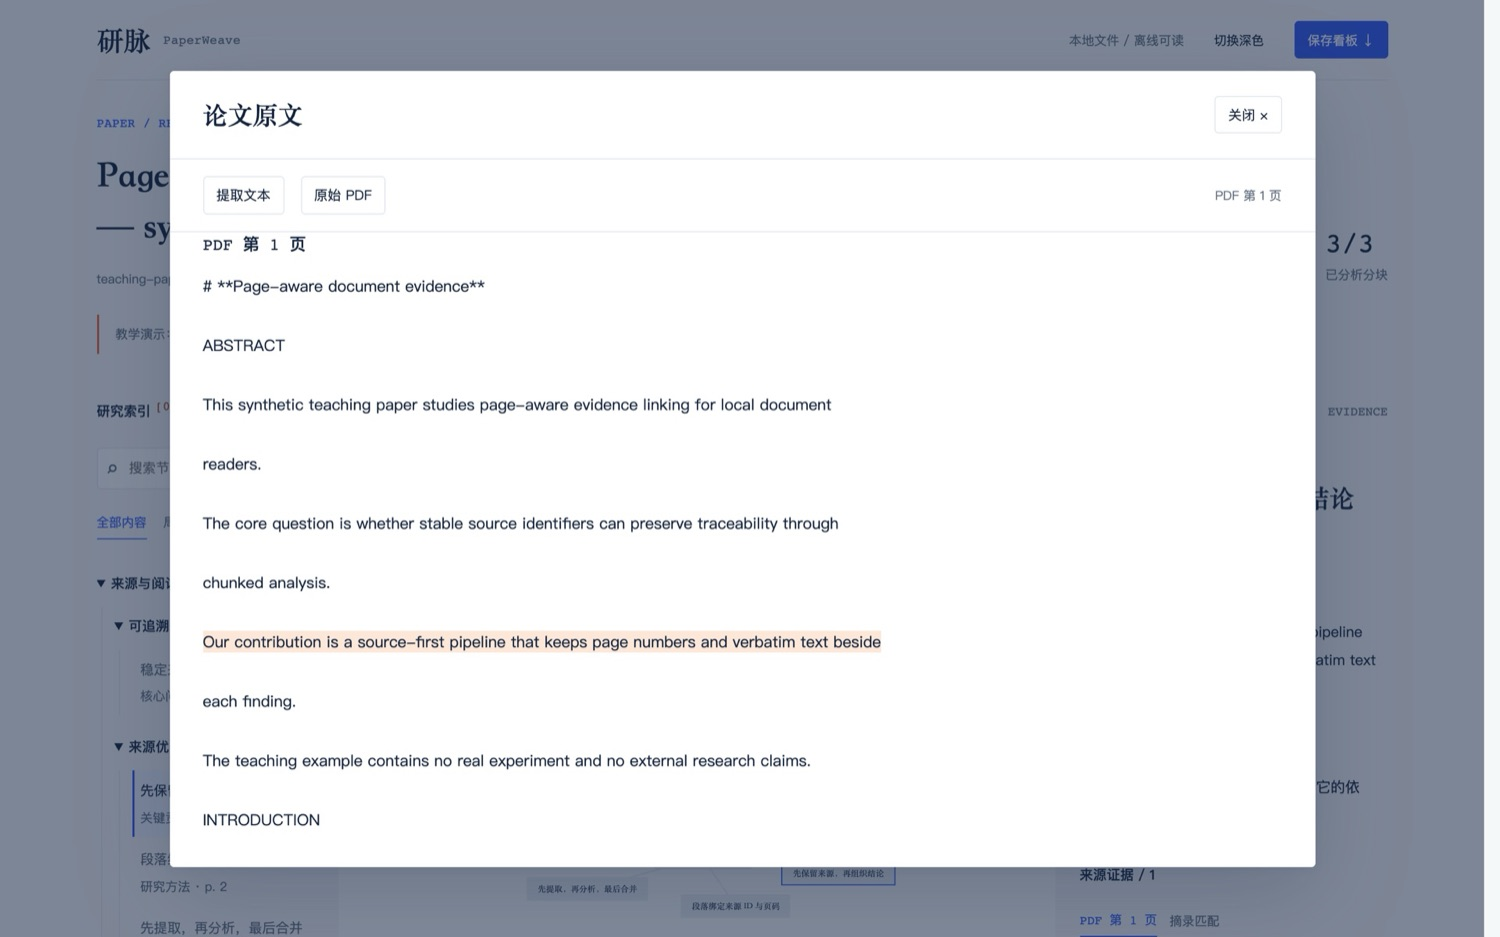
\includegraphics[width=0.42\linewidth]{dash-source}
\caption{证据溯源。左：证据卡片显示物理页码按钮、章节、逐字摘录与匹配状态，“摘录匹配”与“语义待核对”并列提示；右：点击页码后原文对话框按页呈现提取文本，命中摘录高亮，并可切换查看内嵌原始 PDF。}
\label{fig:evidence}
\end{figure*}

\subsection{导图校验与离线看板}

同一主题树生成 Mermaid mindmap 与 flowchart 两种格式，均先经真实 \texttt{mermaid.parse()} 校验\citep{mermaid}，再在 Chromium 中实际渲染为 SVG；标签含非常规字符导致解析失败时，按规则清洗标签结构字符后重试。看板为单文件 HTML：样式、交互脚本、Mermaid 渲染器、结构化数据与预渲染 SVG 全部内嵌，可选内嵌原始 PDF，并以严格内容安全策略约束（\texttt{default-src 'none'}、\texttt{connect-src 'none'}：除内联资源与 data/blob 外禁止一切加载与外联）。自动化测试验证离线模式下无任何 HTTP(S) 请求。

看板交互包括：节点索引与全文关键词搜索、局限与边界筛选、思维导图与结构关系图切换、拖拽平移与滚轮缩放、主题收起展开、节点详情与证据面板（页码按钮跳转原文并高亮摘录）、HTML/SVG/Mermaid/JSON 四种导出、深浅主题切换与移动端适配。

\begin{figure*}[t]
\centering
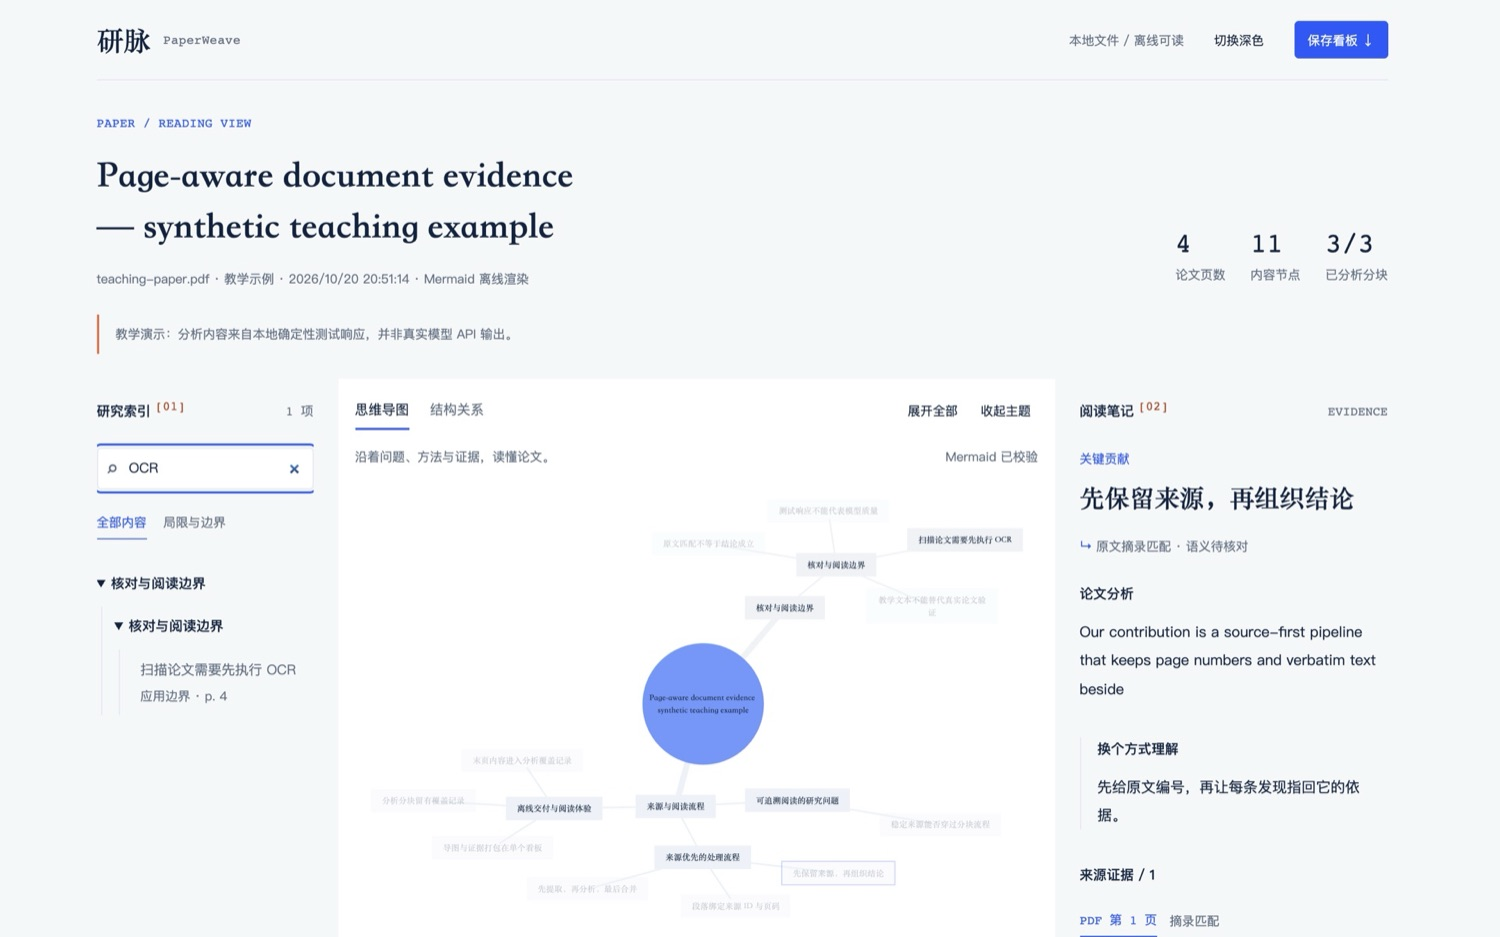
\includegraphics[width=0.42\linewidth]{dash-search}\hfill
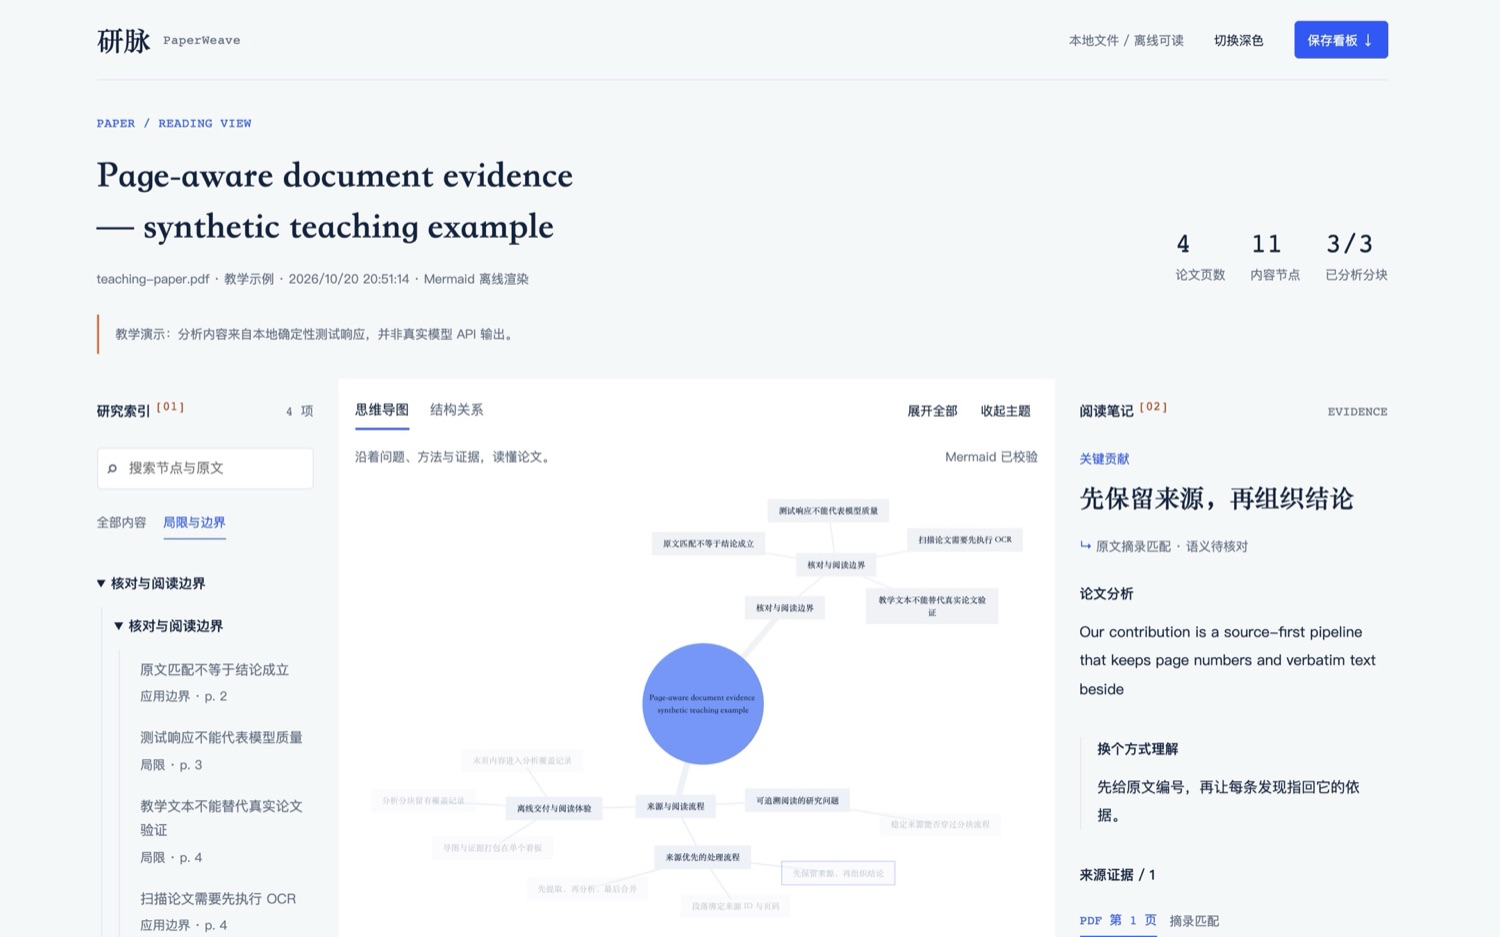
\includegraphics[width=0.42\linewidth]{dash-critical}
\caption{检索与筛选。左：搜索“OCR”时索引收敛为 1 项，导图中不相关节点降低不透明度；右：“局限与边界”筛选仅保留局限性与应用边界类节点，便于快速核查论文自述局限。}
\label{fig:filter}
\end{figure*}

\subsection{本地服务与安全边界}\label{sec:security}

威胁模型覆盖三类攻击面。其一，\textbf{恶意论文文本}：论文内容可能内嵌指令式文本试图操纵模型；系统提示将其声明为数据，模型输出仅按固定 JSON 模式解析，自由文本不进入任何执行路径。其二，\textbf{本机服务暴露}：上传服务仅监听回环地址，校验 Host 与 Origin 头以阻断跨站请求与 DNS 重绑定；并发任务上限 3 个，单文件上限 80 MB，结果文件按白名单路由，杜绝路径穿越。其三，\textbf{凭据泄漏}：API Key 仅经环境变量或 \texttt{.env} 注入，不写入源码、日志与导出文件；认证失败的响应正文不落盘。

\subsection{配置与可复现性}

全部行为参数集中于八个环境变量（表~\ref{tab:config}），程序启动时校验取值边界，非法配置直接报错并给出中文原因。模型协议固定为 Chat Completions，不发送特定供应商才支持的参数，因此可无差别切换 DeepSeek\citep{deepseek2024v3}、本地开源模型或本报告使用的确定性模拟接口。

\begin{table}[t]
\centering
\small
\setlength{\tabcolsep}{3pt}
\begin{tabular}{@{}p{0.40\linewidth}p{0.27\linewidth}p{0.15\linewidth}@{}}
\toprule
\textbf{变量} & \textbf{取值范围} & \textbf{默认} \\
\midrule
LLM\_BASE\_URL & HTTP(S) 地址 & 必填 \\
LLM\_API\_KEY & 非空，不落盘 & 必填 \\
LLM\_MODEL & 非占位符 & 必填 \\
CHUNK\_CHARS & 2000--24000 & 10000 \\
LLM\_MAX\_TOKENS & 512--32000 & 5000 \\
LLM\_TIMEOUT & $>0$ 秒 & 180 \\
LLM\_RETRIES & 0--5 & 2 \\
EMBED\_PDF & 0 / 1 & 1 \\
\bottomrule
\end{tabular}
\caption{环境配置项与启动时校验的取值边界。}
\label{tab:config}
\end{table}

\begin{figure*}[t]
\centering
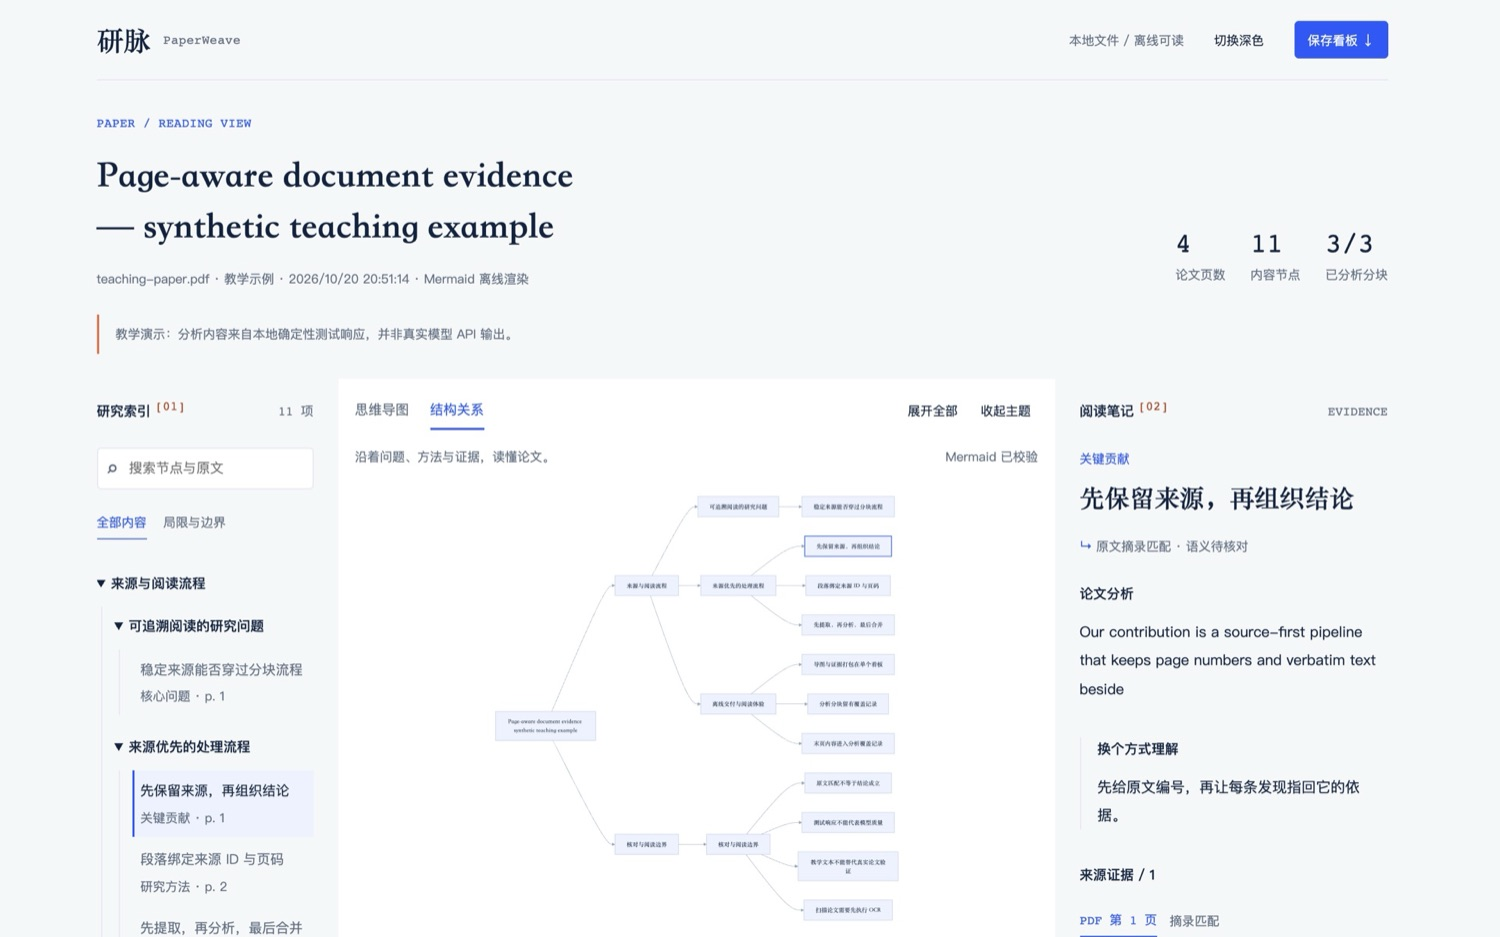
\includegraphics[width=0.42\linewidth]{dash-flowchart}\hfill
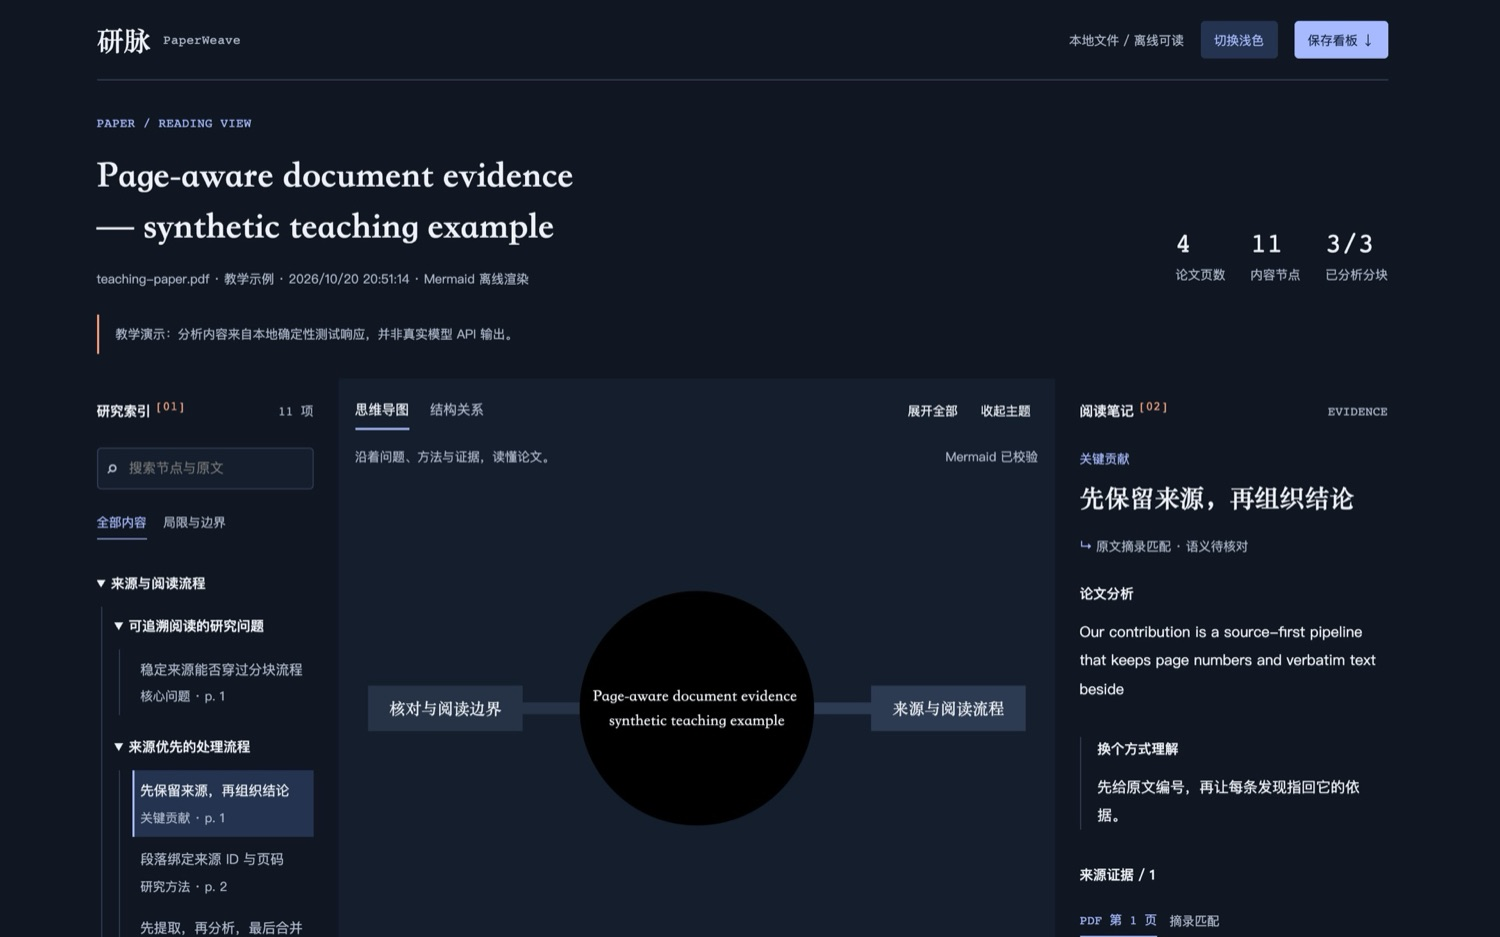
\includegraphics[width=0.42\linewidth]{dash-dark}
\caption{视图切换。左：结构关系图以有向层级呈现同一主题树，连线仅表示归属；右：深色主题下导图与面板同步重渲染，Mermaid 校验状态实时显示。}
\label{fig:views}
\end{figure*}

\section{实现与测试}\label{sec:test}

\subsection{模块构成}\label{sec:modules}

\begin{table}[t]
\centering
\small
\setlength{\tabcolsep}{3pt}
\begin{tabular}{@{}p{0.23\linewidth}c p{0.36\linewidth}p{0.14\linewidth}@{}}
\toprule
\textbf{模块} & \textbf{行数} & \textbf{职责} & \textbf{来源} \\
\midrule
parser.py & 106 & 页级提取、标题识别、来源分块 & 集成 \\
analysis.py & 126 & 校验、匹配、去重、归纳 & 新增 \\
llm.py & 68 & 协议客户端、JSON 修复 & 新增 \\
pipeline.py & 79 & 流程编排、完整性断言 & 新增 \\
render.py & 67 & 导图编译校验、看板导出 & 改造 \\
server.py & 95 & 上传服务、安全中间件 & 新增 \\
config.py & 40 & 配置与边界校验 & 新增 \\
vendor/ & 177 & 数据模型、章节、导图编译 & 复用 \\
\bottomrule
\end{tabular}
\caption{代码构成（合计约 800 行）。\texttt{vendor/} 为 ScholarFlow 与 mindmap-generator 的锁定改造成果，原始授权文本随源码保留。}
\label{tab:modules}
\end{table}

表~\ref{tab:modules} 给出模块构成。第三方复用均锁定上游 commit 并随仓库保留许可文本；分析、协议、编排与安全相关逻辑均为新增，便于审计。

\subsection{自动化测试}

测试套件共 16 项，全部通过（macOS 15 / Python 3.14 与 Windows / Python 3.12 双环境实测）。表~\ref{tab:tests} 按验证目标归纳。其中浏览器级上传流程测试以确定性模拟接口\footnote{模拟响应复用教学规则，仅覆盖教学样例关键词，不代表真实模型质量；接口实现随源码发布于 \texttt{scripts/mock\_llm.py}。}替代真实模型，经 uvicorn 临时端口与 Playwright 自动完成“上传 PDF $\rightarrow$ 任务轮询 $\rightarrow$ 打开看板 $\rightarrow$ 断言 SVG 渲染”全流程；界面回归组覆盖改版后的视觉与可访问性要求（按钮触达区域不小于 44\,px、表单字号不小于 16\,px、长文件名不破坏布局、配置错误可恢复）。

\begin{table}[t]
\centering
\small
\begin{tabular}{@{}p{0.27\linewidth}p{0.61\linewidth}@{}}
\toprule
\textbf{验证目标} & \textbf{测试要点} \\
\midrule
全文覆盖（1） & 分块无截断；末页内容进入导图 \\
证据核验（1） & 伪造摘录标记为未匹配；证据须归属当前块 \\
合并安全（2） & 树完整保留；语义相反的结论不合并 \\
异常处理（1） & 加密/扫描 PDF 给出可操作错误 \\
协议健壮（2） & 非法 JSON 修复；密钥脱敏；401 不泄露正文 \\
导图安全（1） & 标签注入字符被清除 \\
上传流程（1） & 浏览器级：上传 $\rightarrow$ 轮询 $\rightarrow$ 看板打开 \\
离线交互（2） & 断网渲染、节点点击、四种导出、移动端 \\
界面回归（2） & 长文件名、可恢复错误、键盘筛选、触达区域 \\
访问控制（1） & 跨站请求 403；结果文件白名单 \\
\bottomrule
\end{tabular}
\caption{自动化测试覆盖（16 项全部通过，括号内为用例数）。}
\label{tab:tests}
\end{table}

\subsection{陌生论文与离线核查}

以公开论文《Attention Is All You Need》作为开发中不可见的真实双栏 PDF 进行抽取核查：15 页全部提取成功，254 个来源片段全部恰好分配至 7 个分析块，第 14 页文字不足的警告被正确保留而非掩盖，末页内容进入覆盖记录。离线方面，对生成的看板以浏览器离线上下文加载，外部资源请求计数为 0；看板体积约 2.8 MB（内嵌原始 PDF 时），可在移动端正常滚动与缩放。

\subsection{调用与成本模型}

模型调用次数可静态估计：$N_{\text{calls}} = C + R + F$，其中 $C$ 为分析块数，$R$ 为主题归纳批次数（每轮不超过 $\lceil n/24 \rceil$，轮数由分支因子 8 决定），$F\in\{0,1\}$ 为末轮小批量归纳；另有至多 $2C$ 次结构修复重试。输入开销与全文长度线性相关（每块约 \texttt{CHUNK\_CHARS} 字符），输出以 \texttt{LLM\_MAX\_TOKENS} 为上界。教学样例实测：4 页、46 个来源块、3 个分析块、11 个节点，共 5 次调用（3 次分析 + 2 次归纳），无修复重试，与该模型一致。

\subsection{端到端界面测试}

我们在浏览器中对 12 项关键功能逐一操作并截图（图~\ref{fig:upload}--\ref{fig:mobile}）：配置检测、文件选择、进度反馈、完成跳转、导图渲染、节点选择、证据定位、原文高亮、关键词搜索、局限性筛选、结构图切换、深色主题、主题折叠与移动端布局，全部符合预期。测试经本地模拟模型接口驱动真实上传流程完成，看板由该次运行实际生成而非预置文件。界面近期按“克制的科学编辑风格”完成改版——单一蓝色主色、衬线标题、编号栏目（研究索引 / 阅读笔记）——本报告全部截图均为改版后实测。

\begin{figure}[t]
\centering
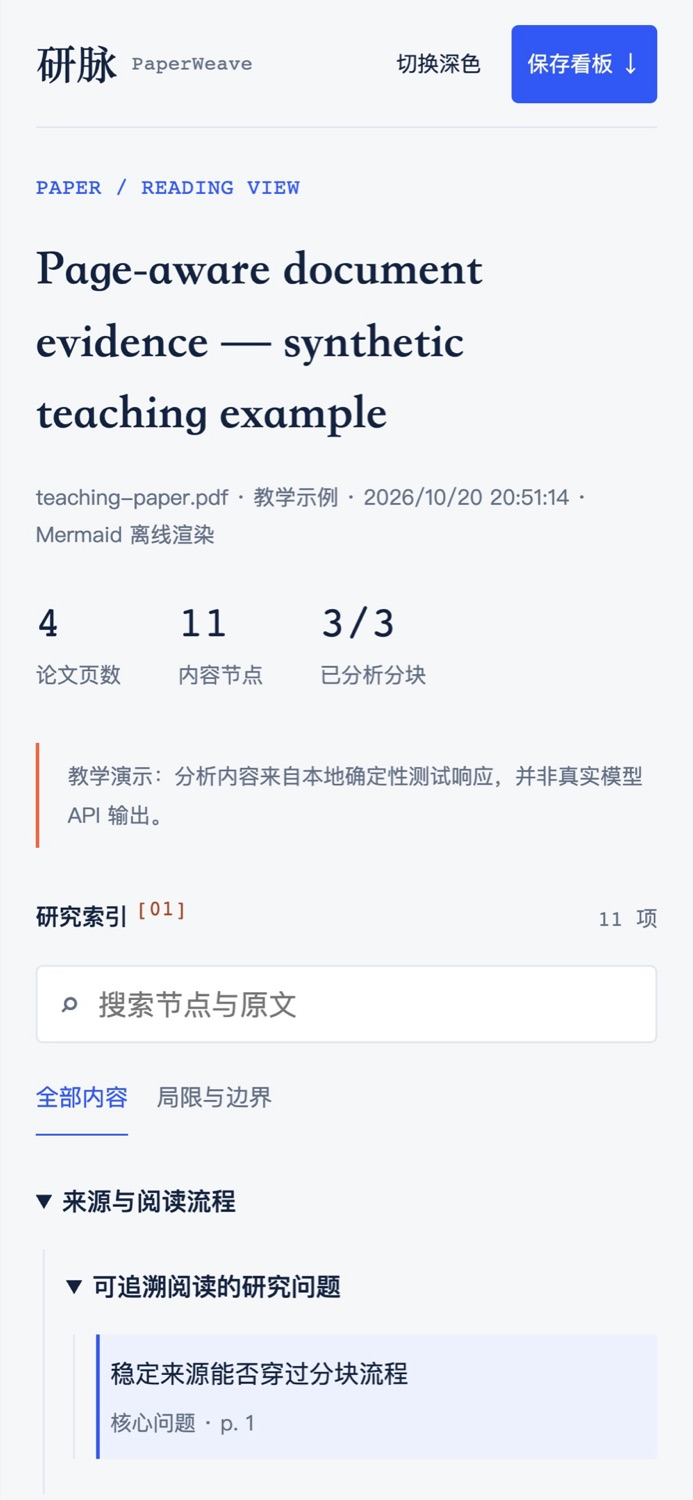
\includegraphics[width=0.62\linewidth]{dash-mobile}
\caption{移动端（390\,pt 视口）：三栏折叠为单列纵向排布，索引、导图与详情仍可独立操作，无横向溢出。}
\label{fig:mobile}
\end{figure}

\section{与比赛要求的对照}

\begin{table}[t]
\centering
\small
\setlength{\tabcolsep}{3pt}
\begin{tabular}{@{}p{0.20\linewidth}c p{0.55\linewidth}@{}}
\toprule
\textbf{评审维度} & \textbf{分值} & \textbf{状态与依据} \\
\midrule
一键跑通 & 30 & 已达成：命令行与上传界面均一次触发全流程 \\
解析准确 & 25 & 机制就绪并经真实双栏 PDF 抽取核查；语义质量待真实模型验收 \\
看板可用 & 20 & 已达成：离线 0 外部请求，交互齐全 \\
内容深度 & 20 & 已实现：页码/章节/摘录溯源、批判性标注、通俗解释 \\
稳定鲁棒 & 15 & 已实现：JSON 修复、网络重试、导图规则修复、完整性断言 \\
工程规范 & 10 & 已达成：文档完备、密钥不落盘、依赖可复现 \\
\bottomrule
\end{tabular}
\caption{与大赛评审维度的对照（合计 120 分）。}
\label{tab:rubric}
\end{table}

表~\ref{tab:rubric} 对照大赛评审维度给出状态。基础部分（提取、分析、导图、看板、一键化）全部达成；提高部分中页码溯源、搜索、导图切换、导出、主题切换、语法自动修复与读者友好解释均已实现，未声称完成的包括图像公式理解、自动 OCR 与独立语义事实核验。

\section{局限与展望}

系统目前存在四点局限。（1）\textbf{模型质量未经验收}：全部定量结果基于确定性模拟响应或抽取层核查，接入主办方 DeepSeek V4 Pro 后的科学分析准确率仍需人工核验；（2）\textbf{文本型 PDF 边界}：扫描件与图片型公式超出基础承诺，系统以显式警告而非静默降级处理；（3）\textbf{摘录匹配非蕴含判定}：证据核验只能确认引文存在，结论正确性仍需读者结合上下文判断，接入独立的蕴含核验通道是下一步方向；（4）\textbf{跨平台验证范围}：macOS 环境为本轮补充实测，正式提交材料仍以已声明的 Windows/Python~3.12 组合为准。此外，模拟接口仅覆盖教学样例关键词，对真实模型行为的回归价值有限，未来可扩充为基于录制响应的更广覆盖。

\section{结论}

研脉系统以来源块与证据核验为中心组织整条流水线，将“模型会出错”作为设计前提而非异常路径，实现了从论文 PDF 到证据可溯、可离线使用的思维导图看板的一键转换。16 项自动化测试与 12 项界面功能测试全部通过，陌生论文抽取与离线场景核查未发现阻断性缺陷。系统已具备比赛基础部分的完整能力，剩余工作集中于真实模型接入后的质量验收。

\bibliography{custom}

\end{document}
